\documentclass{article}
\usepackage[utf8]{inputenc}
\usepackage{amsthm}
\usepackage{amsmath}
\usepackage{amssymb}
\usepackage{enumitem}
\usepackage{float}
\usepackage{graphicx}
\setlength{\parindent}{0em}
\setlength{\parskip}{1em}
\usepackage{fixltx2e}
\newcommand{\Mod}[1]{\ (\mathrm{mod}\ #1)}
\usepackage{mathabx}
\DeclareMathOperator{\tr}{tr}
\usepackage{geometry}
\graphicspath{ {./graphics/} }
 \geometry{
 a4paper,
 total={170mm,257mm},
 left=20mm,
 top=20mm,
 }

\newenvironment{QandA}{\begin{enumerate}[label=\bfseries\alph*.]\bfseries}
                      {\end{enumerate}}
\newenvironment{answered}{\par\normalfont}{}

\title{Calculus 18/19 Sem 1 Suggested Answers}

\author{\makebox[.9\textwidth]{NUS LaTeXify Proj Team}}
\date{Updated: 28 December 2019}

\begin{document}

\maketitle

Done by: Yip Jung Hon and Pan Jing Bin
\hline

\subsubsection*{Question 1}
\begin{enumerate}[label=\roman*)]
    \item Increasing on $(5, \infty)$, decreasing on $(-\infty, 5)$.
    \begin{flalign*}
        f'(x)=\frac{6x-30}{5(x-6)^{4/5}}&&
    \end{flalign*}
    When $f'(x) >0, 6x-30>0 \implies x>5$. When $f'(x)<0 \implies x<5$.
    We also check the points where $f'(x)$ is undefined.
    
    \begin{center}
         \begin{tabular}{||c c c||} 
         \hline
         $x$ & 6^- & 6^+ \\
         \hline\hline
         $f'(x)$ & +ve & +ve \\ 
         \hline
        \end{tabular}
    \end{center}
    
    \item Checking the point at $x=5$ gives us that it is a local min.
    
    \begin{center}
         \begin{tabular}{||c c c||} 
         \hline
         $x$ & 5^- & 5^+ \\
         \hline\hline
         $f'(x)$ & -ve & +ve \\ 
         \hline
        \end{tabular}
    \end{center}
    
    Local min occurs at $(5, -5)$ and there is no local max.
    
    \item Concave up when $(-\infty,6)$ and $(10, \infty)$ and concave down when $(6,10)$.
    \begin{flalign*}
        f''(x)=\frac{6x-60}{25(x-6)^{1/5}}&&
    \end{flalign*}
    When $f''(x)>0$, one needs to have $6x-60>0$ or $x-6>0 \implies x>10$ or $x>6 \implies x>10$. One could also have $6x-60<0$ or $x-6<0 \implies x<10$ or $x<6 \implies x<6$.
    
    When $f''(x)<0$, one needs to have $6x-60<0$ or $x-6>0 \implies x<10$ or $x>6 \implies 6<x<10$. Alternatively, $6x-60>0$ or $x-6<0 \implies x>10$ or $x<6$, but that's impossible.
    
    \item Inflection points are $x=6, 10$ as that is when the graph changes concavity.
\end{enumerate}
\pagebreak

\textbf{Question 2}
\begin{enumerate}[label=\alph*)]
    \item $\lim_{x \rightarrow 1^+} \frac{x+3}{x-1}= \infty$ iff $\forall M >0, \exists \delta>0$ such that $0<x-1<\delta \implies f(x) > M$.
    
    Rough work: $f(x)>M \implies \frac{x+3}{x-1}>M$. So whichever $\delta$ we pick must ensure $\frac{x+3}{x-1}>M$. Intuitively, what this means is that when $0<x-1<\delta$, we must find a lower bound for $x+3$ and an upper bound for $x-1$ (which is $\delta$) so that we can establish the following inequality:
    \begin{flalign*}
        \frac{x+3}{x-1}>\frac{\text{Lower bound for ($x$+3)}}{x-1}>\frac{\text{Lower bound for ($x$+3)}}{\delta}>M&&
    \end{flalign*}
    Assume $0<x<1$ is sufficient, then we have $0<x<2 \implies 3<x+3<5$, so the lower bound for $x+3$ is 3.
    
    Proof: Picking $\delta=\min\{1,\frac{3}{M}\}$ is sufficient.
    If $M>3$, pick $\delta=\frac{3}{M}<1$.
    So one has:
    \begin{flalign*}
        \frac{x+3}{x-1}>\frac{3}{x-1}>\frac{3}{3/M}=M&&
    \end{flalign*}
    If $M\leq 3$, pick $\delta=1$.
    \begin{flalign*}
        \frac{x+3}{x-1}>\frac{3}{x-1}>\frac{3}{1}=3\geq M&&
    \end{flalign*}
    
    \item 6
    \begin{align*}
        \lim_{x \rightarrow \infty} \left[ \frac{1}{3} \left( 3^{1/x}+8^{1/x}+9^{1/x}) \right) \right]^x &= \lim_{u \rightarrow 0} \left[ \frac{1}{3} \left( 3^{u}+8^{u}+9^{u}) \right) \right]^{1/u} \hspace{25pt} \text{(Let $u=1/x$)}\\
        &=\exp \left( {\lim_{u \rightarrow 0} \frac{\ln(\frac{1}{3}[3^u+8^u+9^u])}{u}}\right)\ \ \text{(Use L'hospital rule, top and bottom go to 0)} \\
        &=\exp \left( {\lim_{u \rightarrow 0}  \frac{3^u\ln3+8^u\ln8+9^u\ln9}{3^u+8^u+9^u}}\right) \\
        &=\exp \left( \frac{\ln3+\ln8+\ln9}{3} \right)\\
        &=\exp \left(\ln216^{1/3} \right) \\
        &=6
    \end{align*}
    \item $y=(\frac{1}{x})^{\ln x} \implies \ln y = (\ln x)(\ln \frac{1}{x})$.
    
    Implicitly differenciating:
    \begin{align*}
        &\frac{1}{y}\frac{dy}{dx}=(\ln x)(\frac{1}{1/x})(-\frac{1}{x^2}) + \ln(\frac{1}{x})(\frac{1}{x}) \\
        &\frac{1}{y}\frac{dy}{dx}=-\frac{1}{x}\ln x +\frac{1}{x} \ln (\frac{1}{x}) = -\frac{2}{x}\ln x  \\
    \intertext{When $x=e, y=1/e$. We have:}
        &\frac{1}{1/e}\frac{dy}{dx} = -\frac{2}{e}\ln e  \\
        & e\frac{dy}{dx}=-\frac{2}{e}\\
        & \frac{dy}{dx}=-\frac{2}{e^2}
    \intertext{Equation of tangent:}
        &\frac{y-\frac{1}{e}}{x-e}=\frac{-2}{e^2}\\
        &y=-\frac{2x}{e^2}+\frac{3}{e}
    \end{align*}
\end{enumerate}
\pagebreak

\textbf{Question 3} $D=\sqrt{3}R, W=R$.

We know:
\begin{align*}
    &(\frac{W}{2})^2+(\frac{D}{2})^2=R^2 \\
    &W^2=4R^2-D^2 
\intertext{We model stiffness as:}
    &S=kWD^3 \\
    &S^2=k^2W^2D^6 \\
    &S^2=k^2(4R^2-D^2)D^6&&
\intertext{Implicitly differentiating w.r.t $D$,}
    &2S\frac{dS}{dD}=k^2(24R^2D^5-8D^7)
\end{align*}
Setting $dS/dD=0$, we have $D=0$ or $D=\pm \sqrt{3}R$. Rejecting 0 and $-\sqrt{3}R$, we check for maxima:
    \begin{center}
         \begin{tabular}{||c c c||} 
         \hline
         $D$ & $\sqrt{3}R^-$ & $\sqrt{3}R^+$ \\
         \hline\hline
         $dS/dD$ & +ve & -ve \\ 
         \hline
        \end{tabular}
    \end{center}
When $D=\sqrt{3}R, W=R$. 

\subsubsection*{Question 4}
\begin{enumerate}[label=\roman*)]
\item Let $y=f(x)$. Then $x=g(y)$.
Using inverse differentiation: $g'(y)=\frac{1}{f'(x)}=[f'(x)]^{-1} $.
Differentiating this with respect to $x$:
\begin{align*}
    g''(y)&f'(x) = -[f'(x)]^{-2}f''(x)\\
    g''(y)&=-\frac{f''(x)}{[f'(x)]^3}\\
    &=-\frac{f''(g(y))}{[f'(g(y))]^3}
\end{align*}

\item From part(i), we have: $g''(y)=-f''(x)[f'(x)]^{-3}$\\\\
Differentiating with respect to $x$:
\begin{flalign*}
    g'''(y)f'(x)&=-f'''(x)[f'(x)]^{-3} - (-3)(f''(x))[f'(x)]^{-4}(f''(x))\\
    &=[f'(x)]^{-4}[-f'''(x)f'(x)+3[f''(x)]^2]\\
    g'''(y) &= \frac{3[f''(x)]^2-f'''(x)f'(x)}{[f'(x)]^5}\\
    &=\frac{3[f''(g(y))]^2-f'(g(y))f'''(g(y))}{[f'(g(y))]^5}
\end{flalign*}
\end{enumerate}

\pagebreak
\subsubsection*{Question 5}
\begin{enumerate}[label=\alph*)]
\item(i) Using washer method:
\begin{align*}
    \text{Volume} &= \int^1_0 \pi(2)^2dx-\int^1_0 \pi y^2dx\\
    &= 4\pi x \big|^1_0 - \pi \int^1_0 \frac{1}{(1+x)^4}dx\\
    &=4\pi - \pi[{\frac{-1}{3(1+x)^3}}\big|^1_0]\\
    &=4\pi + \frac{\pi}{3}(\frac{1}{8}-\frac{1}{1})\\
    &=4\pi - \frac{7\pi}{24}\\
    &=\frac{89\pi}{24}
\end{align*}
(ii) Using method of cylindrical shells:
\begin{align*}
    \text{Volume} &= \int^1_0 2\pi(2-x)(2)dx - \int^1_0 2\pi(2-x)(\frac{1}{1+x})^2dx\\
    &=4\pi(2x-\frac{1}{2}x^2)\big|^1_0 - 2\pi\int^1_0\frac{2-x}{x^2+2x+1}dx\\
    &=6\pi - 2\pi\int^1_0 -\frac{1}{2}[\frac{2x+2}{(1+x)^2}] + \frac{3}{(1+x)^2}dx\\
    &=6\pi - 2\pi[-\ln{(1+x)} - \frac{3}{1+x}]\big|^1_0\\
    &=6\pi - 2\pi[-\ln2 -\frac{3}{2}+\ln1+\frac{3}{1}]\\
    &=3\pi +2\pi\ln2
\end{align*}
    \item Arc length = $\int^b_0\sqrt{1+(f'(x))^2}dx$.
\begin{align*}
    &\int^b_0\sqrt{1+(f'(x))^2}dx = b + \frac{2}{3}b^3
\intertext{Differentiating with respect to $b$:}
    &\sqrt{1+(f'(b))^2}=1+2b^2\\
    &1+(f'(b))^2=1+4b^2+4b^4\\
    &f'(b) = \pm\sqrt{4b^2+4b^4}
\end{align*}

Note that in the case of $f'(b) = -\sqrt{4b^2+4b^4}$, $\lim_{b\to\infty} f'(b) = -\infty$.

This implies that $\lim_{b\to\infty} f(b) = -\infty$ which contradicts the given condition that $f$ is a nonnegative function. Thus we reject the case of $f'(b) = -\sqrt{4b^2+4b^4}$.

    \begin{align*}
        f'(b)& = 2b\sqrt{b^2+1}\\
        f(b) &= \int2b\sqrt{b^2+1}db\\
        &=\int\sqrt{u+1}du\ \ \text{(Substitute $u = b^2$,$\frac{du}{db} = 2b$)}\\
        &=\frac{2}{3}(u+1)^{\frac{3}{2}} + C\\
        &=\frac{2}{3}(b^2+1)^{\frac{3}{2}} + C\\
        f(0) &= \frac{2}{3} \implies \frac{2}{3} = \frac{2}{3}(1)^{\frac{3}{2}} + C \implies C=0 \\
        f(x)&=\frac{2}{3}(x^2+1)^{\frac{3}{2}}
    \end{align*}
\end{enumerate}
\pagebreak

\subsubsection*{Question 6}
\begin{enumerate}[label=\alph*)]
\item
\begin{flalign*}
    \int\frac{x}{\sqrt{9+8x^2-x^4}}dx &= \frac{1}{2}\int\frac{1}{\sqrt{9+8u-u^2}}du \ \ \text{(Use substitution $u=x^2,\frac{du}{dx}=2x)$}\\
    &=\frac{1}{2}\int\frac{1}{\sqrt{25-(u^2-8u+16)}}du\\
    &=\frac{1}{2}\int\frac{1}{\sqrt{25-(u-4)^2}}du\\
    &=\frac{1}{2}\int\frac{5\cos{v}}{\sqrt{25-25\sin{^2v}}}dv\ \ \text{(Use substitution $5\sin{v}=u-4,\frac{du}{dv}=5\cos{v}$})\\
    &=\frac{1}{2}\int\frac{5\cos{v}}{5\cos{v}}dv\\
    &=\frac{1}{2}\int1dv\\
    &=\frac{1}{2}v+C\\
    &=\frac{1}{2}\sin{^{-1}\frac{u-4}{5}}+C\\
    &=\frac{1}{2}\sin{^{-1}\frac{x^2-4}{5}}+C
\end{flalign*}
\item Consider 2 cases:

Case 1: $p=-1$.
\begin{flalign*}
    &\int^1_0x^{-1}\ln{x}dx = (\ln{x})^2\big|^1_0 - \int^1_0x^{-1}\ln{x}dx\\
    &2\int^1_0x^{-1}\ln{x}dx = (\ln{x})^2\big|^1_0\\
    &\int^1_0x^{-1}\ln{x}dx = \frac{1}{2}(\ln{x})^2\big|^1_0
\intertext{Clearly the integral does not converge as $\lim_{x\to0}\ln x \rightarrow -\infty$.}
\intertext{Case 2: $p\neq-1$.}
    \int^1_0 x^p\ln{x}dx &= \frac{x^{p+1}}{p+1}\ln{x}\big|^1_0-\int^1_0\frac{x^{p+1}}{p+1}(\frac{1}{x})dx\\
    &=\frac{x^{p+1}}{p+1}\ln{x}\big|^1_0-\int^1_0\frac{x^p}{p+1}dx\\
    &=\frac{x^{p+1}}{p+1}\ln{x}\big|^1_0 - \frac{x^{p+1}}{(p+1)^2}\big|^1_0 \\
    &=\frac{x^{p+1}}{p+1}\ln{x}\big|^1_0 - \frac{1}{(p+1)^2} \\
    &=0 - \lim_{x\to0}\frac{x^{p+1}\ln{x}}{p+1} - \frac{1}{(p+1)^2}
\end{flalign*}
Note that $\frac{1}{(p+1)^2}$ which is a finite value as $p \neq -1$. For the integral to converge, $\lim_{x\to0}\frac{x^{p+1}\ln{x}}{p+1}$ must also be some finite value. We note that as $x \to 0$, $\ln x \to -\infty$, so intuitively, for the limit to exist, $x^{1+p}$ should go to 0. Now we claim that $\lim_{x\rightarrow0}{(x^{1+p}\ln{x})}$ converges iff $p>-1$.

% If the integral converges, then $\lim_{x\to0}\frac{x^{p+1}\ln{x}}{p+1}$ exists.
% As $x\to0, \ln{x}\to -\infty \implies x^{p+1}\to0 \implies p>-1$\\
Proof:

If $p<-1$, we would have $\lim_{x\rightarrow0}x^{1+p} \to \infty$ and $\lim_{x\rightarrow0}\ln{x} \to -\infty$, and thus their product cannot be finite.

But when $p>-1$:\\
\begin{flalign*}
    \lim_{x\to0}\frac{x^{p+1}\ln{x}}{p+1} &= \frac{1}{p+1}\lim_{x\to0}\frac{\ln{x}}{x^{-p-1}}[\frac{-\infty}{\infty}]\\
    &= \frac{1}{p+1}\lim_{x\to0}\frac{\frac{1}{x}}{(-p-1)x^{-p-2}} \ \ \text{(By L'Hopital's rule)}\\
    &= \frac{1}{p+1}\lim_{x\to0}\frac{x^{p+1}}{(-p-1)} \\
    &= 0
\end{flalign*}
Thus when $p>-1,\frac{x^{p+1}}{p+1}\ln{x}\big|^1_0=0$.

The integral converges when $p>-1$ and $\int^1_0 x^p\ln{x}dx = \frac{x^{p+1}}{p+1}\ln{x}\big|^1_0 - \frac{x^{p+1}}{(p+1)^2}\big|^1_0 = -\frac{1}{(p+1)^2}$.

\end{enumerate}
\pagebreak

\subsubsection*{Question 7}
\begin{enumerate}[label=\alph*)]
\item Find the integrating factor:
\begin{align*}
    e^{\int \frac{2x+1}{x}dx} &= e^{\int 2+\frac{1}{x}dx}\\
    &= e^{2x+\ln{x}}\\
    &= xe^{2x} \\ 
    xe^{2x}y&=\int xe^{2x}(2x)dx\\
    &=\int 2x^2e^{2x}dx\\
    &=x^2e^{2x}-\int 2xe^{2x}dx\\
    &=x^2e^{2x}-xe^{2x}+\int e^{2x}dx\\
    &=x^2e^{2x}-xe^{2x}+\frac{1}{2}e^{2x}+C \\
    y&=x-1+\frac{1}{2x}+\frac{C}{xe^{2x}}
\intertext{When $x=1,y=1$,}
    &1=1-1+\frac{1}{2}+\frac{C}{e^2}\\
    &C=\frac{e^2}{2}\\
    &y=x-1+\frac{1}{2x}+\frac{e^2}{2xe^{2x}}
\end{align*}
\item (i)
\begin{flalign*}
    &\frac{dQ}{dt}=a-bQ\\
    &\frac{1}{a-bQ}\frac{dQ}{dt}=1\\
    &\int\frac{1}{a-bQ}dQ=\int1dt\\
    &-\frac{1}{b}\ln|a-bQ|=t+C\\
    &|a-bQ|=e^{-bt-bc}\\
    &a-bQ=Ae^{-bt} \ \ \text{(where $A = \pm e^{-bc}$)}\\
    &Q=\frac{a-Ae^{-bt}}{b}
\end{flalign*}
As $t\to\infty,e^{-bt}\to0,Q\to\frac{a}{b}$.

Limiting concentration = $\frac{a}{b}$.
(ii) When $t=0,Q=0$.
\begin{align*}
    &0=\frac{a-Ae^0}{b}\implies a-A=0 \implies A=a\\
    &Q=\frac{a-ae^{-bt}}{b}
\intertext{When Q =$\frac{1}{2}(\frac{a}{b})$:}
    &\frac{a}{2b}=\frac{a-ae^{-bt}}{b}\\
    &\frac{a}{2}=a-ae^{-bt}\\
    &e^{-bt}=\frac{1}{2}\\
    &bt=-\ln{\frac{1}{2}}\\
    &t=\frac{\ln2}{b}
\end{align*}

\end{enumerate}
\pagebreak


\textbf{Question 8}
\begin{enumerate}[label=\alph*)]
    \item By Rolle's, $\exists c$ such that $f'(c)=0$.
    Take the gradient between 0 and $c$, one has by MVT the existence of point $p_1 \in (0, c)$ such that
    \begin{flalign*}
        f'(p_1)=\frac{f(c)-f(0)}{c-0}=\frac{f(c)}{c} > 0&&
    \end{flalign*}
    Likewise, taking gradient between $c$ and 1, one has by MVT the existence of point $p_2 \in (c, 1)$ such that
    \begin{flalign*}
        f'(p_2)=\frac{f(1)-f(c)}{1-c}=\frac{-f(c)}{1-c} < 0&&
    \end{flalign*}
    By MVT theorem on the graph of $f'(x)$, there exists $p_3 \in (p_1, p_2)$ such that
    \begin{flalign*}
        f''(p_3)=\frac{f'(p_2)-f'(p_1)}{p_2-p_1}<0&&
    \end{flalign*}
    Since $p_2 > p_1$. So there exists a point such that $f''(x)< 0.$
    
    \item The intuitive idea behind the proof is to draw a triangle of gradient $M$ from the point $(1/2, g(1/2))$. Then $g(x)$ must always lie above this triangle, else it would have point which has gradient $>M$.
    
    \begin{figure}[H]
        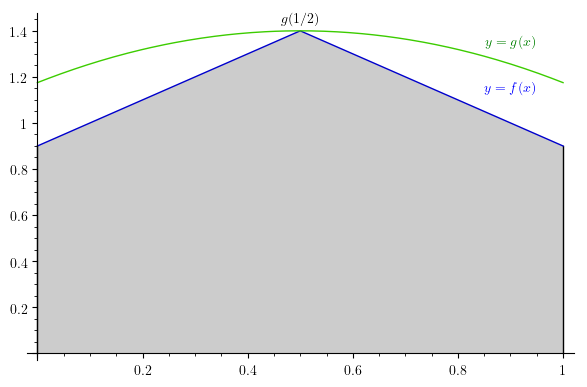
\includegraphics[width=14cm]{q8b.png}
        \centering
        \end{figure}
        
        The area of the shaded trapezium is $g(1/2)-M/4$ and the inequality follows trivially. However, to formalise the proof:
        
        Consider the function defined by:
        \begin{align*}
            f(x) =
            \begin{cases}
                Mx-\frac{1}{2}M+g(1/2),  & \text{if $0\geq x\leq 1/2$} \\
                -Mx+\frac{1}{2}M+g(1/2)  & \text{if $1/2<x \leq 1$}\\
            \end{cases}
        \end{align*}
        $f(x)$ has a maximum point at $(1/2, g(1/2))$. We claim that for all $x$, $f(x) \leq g(x)$. Suppose there exists $c \neq 1/2$ such that $f(c)>g(c)$. WLOG, assume $c < 1/2$. We thus have $\frac{g(1/2)-g(c)}{1/2-c}>M$. By MVT, this implies there exists $p \in (c, 1/2)$ such that $g'(p)>M$, which is a contradiction. Similarly, we can conclude that if $c>1/2$, we have $\frac{g(c)-g(1/2)}{c-1/2}<-M$.
        
        Consider $\int^1_0 f(x) dx$. We have:
        \begin{equation*}
            \int^1_0 f(x) dx=\int^{1/2}_0 Mx-\frac{1}{2}M+g(1/2) \ dx + \int^{1}_{1/2} -Mx+\frac{1}{2}M+g(1/2)\ dx = g(1/2)-M/4
        \end{equation*}
        Since $g(x)\geq f(x)$ for all $x$, one has $\int^1_0 g(x) dx \geq \int^1_0 f(x) dx = g(1/2)-M/4$, which gives the desired inequality. \qed
\end{enumerate}
\end{document}
